\documentclass[12pt,a4paper]{article}
\usepackage{fullpage, listings, footnote, graphicx, floatrow, hyperref, multicol, enumitem, latexsym, placeins}
\setdescription{leftmargin=\parindent,labelindent=\parindent}
\pdfpxdimen=\dimexpr 1 in/72\relax
\lstset{
 	basicstyle=\ttfamily,
	breaklines = true,
	language = bash,
}
\author{Hawk Weisman}
\title{CMPSC440 Laboratory Assignment I}
\date{Monday, January 27th, 2014}
\begin{document}
	\maketitle
	\section{Using screenshots and complete examples, a description of the key features provided by zsh}

		The Z shell, or zsh, is a Unix shell designed primarily for interactive use \footnote{As opposed to shells that are intended primarily as a shall-scripting language.}, although it also includes a full-featured shell-scripting language. zsh supports all of the standard features of a POSIX command-line shell.

		Zsh provides a number of advantages over other Unix shells such as \lstinline{bash}, \lstinline{tcsh}, and \lstinline{csh}. For example, zsh offers inline glob completion, meaning that a user can type a command such as \lstinline{ls L*}, press tab, and zsh will expand the glob to a list of all files beginning with the letter L, as seen in figure \ref{tab}. Furthermore, zsh offers many additional features related to globbing and glob completion --- for example, slashes can be used to match directories and periods used to match files, as in \lstinline{*.*} and \lstinline{*\}, which will match all files and all directories, respectively. The use of these features can be seen in figures \ref{dot} and \ref{slash}. The pattern \lstinline{**/} will expand to match paths with any number of directories of depth from the current location is also a unique feature of zsh's glob-completion system.

		\begin{figure}[ht!]
			
\includegraphics[resolution=72, scale=0.75]{Lab1Images/pretab.png}
			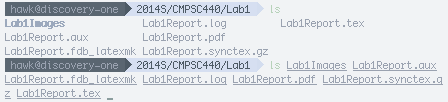
\includegraphics[resolution=72, scale=0.75]{Lab1Images/posttab.png}
			\caption{A zsh glob before and after tab expansion}
			\label{tab}
		\end{figure}

		\begin{figure}[ht!]
			
\includegraphics[resolution=72, scale=0.75]{Lab1Images/predot.png}
			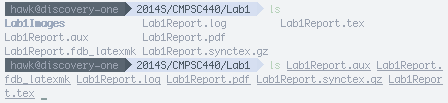
\includegraphics[resolution=72, scale=0.75]{Lab1Images/postdot.png}
			\caption{Using a dot to match files in a zsh glob}
			\label{dot}
		\end{figure}


		\begin{figure}[ht!]
			
\includegraphics[resolution=72, scale=0.75]{Lab1Images/predot.png}
			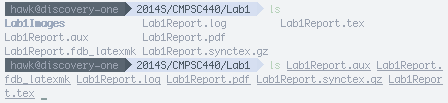
\includegraphics[resolution=72, scale=0.75]{Lab1Images/postdot.png}
			\caption{Using a slash to match directories in a zsh glob}
			\label{slash}
		\end{figure}

		In addition to automatically expanding globs, the Z shell offers a programmable command-autocompletion system. While most modern Unix shells allow users to automatically complete file paths, zsh's tab-completion system offers a number of additional features. For example, it will automatically expand paths where only first letter of each directory is given --- \lstinline{/u/l/b} becomes \lstinline{/usr/local/bin}. Zsh will also autocomplete flags for Unix commands: for example, typing \lstinline{git --} and then pressing tab will display a list of available flags for git, and allow the user to press tab to scroll through the list, as seen in figure \ref{arguments}. Zsh will also autocomplete other Unix commands: typing \lstinline{cd} and then pressing tab will display a list of available directories in the current working directory that the user may then scroll through, while typing the name of a directory will automatically cd to that directory, provided that it is within the current working directory.

		\begin{figure}[ht!]
			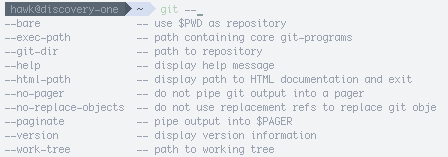
\includegraphics[resolution=72, scale=0.75]{Lab1Images/gittab.png}
			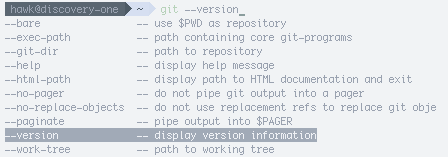
\includegraphics[resolution=72, scale=0.75]{Lab1Images/gitscroll.png}
			\caption{Using zsh tab autocompletion to display and scroll through command-line flags}
			\label{arguments}
		\end{figure}

		Zsh offers a number of features that provide the user a great deal of power to customize the shell. The zsh command prompt is themable, meaning that the user can customize what information the command prompt displays. While many Unix shells provide at least some functionality related to customizing the user's prompt, zsh's is the most full-featured, and allows the use of colors and graphics, as well as the display of additional information about the user's system, such as git repository status, laptop battery life, and internet connection status, collected by running external scripts. Figure \ref{themes} provides examples of zsh themes available from the oh-my-zsh open-source configuration framework. Zsh themes may be distributed as zsh shell script files. Oh-my-zsh also allows users to customize their Z shell environment by installing plugins, zsh script files that add or modify commands, enhance command autocompletion, interface with tools, programming languages, and operating system features, and otherwise modify the shell environment.

		\begin{figure}[ht!]
			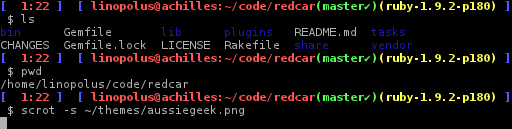
\includegraphics[scale=0.90]{Lab1Images/themes/aussiegeek.png}
			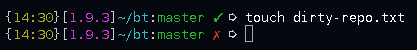
\includegraphics[resolution=72, scale=0.75]{Lab1Images/themes/crunch.png}
			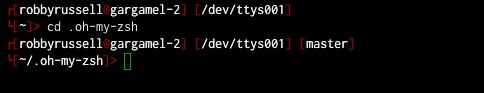
\includegraphics[scale=0.90]{Lab1Images/themes/darkblood.jpg}
			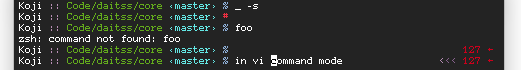
\includegraphics[resolution=72, scale=0.75]{Lab1Images/themes/flazz.png}
			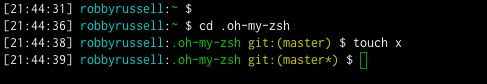
\includegraphics[scale=0.90]{Lab1Images/themes/geoffgarside.jpg}
			\caption{A number of different zsh themes, available through the oh-my-zsh open-source project.}
			\label{themes}
		\end{figure}

	\section{A commentary on the features that zsh provides that your previous shell did not}

		On both Ubuntu and Mac OS X, the default shell is bash. On my laptop, I have been using fish, the \textit{f}riendly \textit{i}nteractive \textit{sh}ell, prior to switching to zsh. Fish offers a number of useful and powerful features, such as automatic suggestion of commands based on the user's command history, a tab-completion system similar to zsh's, and syntax highlighting for commands. However, zsh is much more customizable and expandable than fish, and there are plugins for zsh that will replicate most of the major features of fish --- installing the ``zsh-syntax-highlighting'', ``zsh-history-substring-search'', and ``zsh-autosuggestions'' plugins will essentially transform zsh into fish. Installing these plugins has allowed me to migrate from fish to zsh relatively seamlessly and take advantage of zsh's additional features and improved customization over fish.

		It's also interesting to note that zsh has ``emulation modes'' in which it will emulate the ksh and sh shells, allowing it to run shell scripts written in those languages.

	\section{A tutorial on how to download, install, and configure oh-my-zsh}
		\subsection{Install the oh-my-zsh community-driven framework}

			Oh-my-zsh can be installed automatically using \lstinline{wget} or \lstinline{curl}, by typing \lstinline{wget --no-check-certificate https://raw.github.com/robbyrussell/oh-my-zsh/master/tools/install.sh -O - | sh} or \lstinline{curl -L https://raw.github.com/robbyrussell/oh-my-zsh/master/tools/install.sh | sh}, respectively. It can also be installed manually, by cloning the git repository located at \url{git://github.com/robbyrussell/oh-my-zsh.git} into \verb!~/.oh-my-zsh! and copying the provided config file from the repository using \verb!cp ~/.oh-my-zsh/templates/zshrc.zsh-template ~/.zshrc!.

		\subsection{Change the display of the zsh prompt (e.g., show the user name and host name)}

			Most zsh themes modify the zsh prompt, and users may simply select a theme from those distributed with oh-my-zsh, or write their own theme that displays a prompt that is to their liking. However, if a user wishes to change their zsh prompt without the use of themes, they can do so by setting the \lstinline{PROMPT} variable in their \verb!~/.zshrc! configuration file. Zsh also supports an optional \lstinline{RPROMPT} variable that will display a separate prompt at the right side of the terminal.

			The prompt is modified by setting the \lstinline{PROMPT} and \lstinline{RPROMPT} variables equal to strings containing escape sequences that display various kinds of information. For example, a user who wishes to display their username, host name, and current working directory might add a line similar to \verb!\$PROMPT="%n@%m %~ $"!, which will display a prompt of the form \lstinline{hawk@ewire21-114 ~ $}. The escape character \lstinline{%n} will display the current user's username, while \lstinline{%m} will display the hostname. The \verb!%~! escape character will display the path to the current working directory relative to \verb!/home/member/u/username!. Characters that are not escaped with the \lstinline{%} character will be displayed verbatim. A complete listing of escape characters used to set the zsh prompt is available in the zsh documentation at \\\url{http://zsh.sourceforge.net/Doc/Release/Prompt-Expansion.html}.

		\subsection{Commentary on how to install, configure, and use the following zsh plugins}

			\subsubsection{git}

				The git plugin for zsh is bundled in oh-my-zsh, and is installed automatically if the user installs that framework. It must be enabled by adding it to the list of plugins in the user's \verb$~/.zshrc$. After enabling a plugin, the .zshrc must be re-sourced, either by restarting zsh by typing \lstinline{zsh} and pressing return, or using the command \verb$source ~/.zshrc$. The git plugin for zsh defines the following short aliases for common git commands:
				\begin{description}[leftmargin=3cm, style=sameline]
					\begin{multicols}{2}
						\item[g]{\lstinline!git!}
						\item[gl]{\lstinline!git pull!}
						\item[gca]{\lstinline!git commit -v -a!}
						\item[gcm]{\lstinline!git checkout master!}
						\item[gba]{\lstinline!git branch -a!}
						\item[ga]{\lstinline!git add!}
						\item[grh]{\lstinline!git reset HEAD!}
						\item[gsr]{\lstinline!git svn rebase!}
						\item[gst]{\lstinline!git status!}
						\item[gup]{\lstinline!git fetch && git rebase!}
						\item[gc]{\lstinline!git commit -v!}
						\item[gco]{\lstinline!git checkout!}
						\item[gb]{\lstinline!git branch!}
						\item[gcount]{\lstinline!git shortlog -sn!}
						\item[gss]{\lstinline!git status -s!}
						\item[gm]{\lstinline!git merge!}
						\item[grhh]{\lstinline!git reset HEAD --hard!}
						\item[gsd]{\lstinline!git svn dcommit!}
					\end{multicols}
					\item[glgg]{\lstinline!git log --graph --max-count=5!}
					\item[glg]{\lstinline!git log --stat --max-count=5!}
					\item[ggpush]{\lstinline!git push origin $(current_branch)!}
					\item[ggpnp]{\lstinline!git pull origin $(current_branch) && git push origin $(current_branch)!}
					\item[gpa]{\lstinline!git add .; git commit -m "$1"; git push;!}
					\item[gdv]{\lstinline!git diff -w "$@" | view -!}
					\item[ggpull]{\lstinline!git pull origin $(current_branch)!}
					\item[git-svn-dcommit-push]{\lstinline!git svn dcommit && git push github master:svntrunk!}
				\end{description}

			\subsubsection{web-search}

				The web-search plugin for zsh is also bundled in oh-my-zsh, and can be enabled by adding it to the list of enabled plugins in the user's .zshrc. It allows users to search the internet from the command line using the Google, Bing, and Yahoo search engines. Typing the name of the search engine, followed by a query --- for example, \lstinline{google oh-my-zsh} --- will open a search results page from that search engine in the user's default browser.

			\subsubsection{wd}

				Wd, the ``warp directory'' plugin, allows users to define ``warp points'', directories that may be jumped to without using their full paths. It is also bundled with oh-my-zsh, and may be enabled by adding \lstinline{wd} to the list of enabled plugins in the user's .zshrc.

				A warp point to the current working directory may be created using the command \lstinline{wd add <warp point name>}. The user may then type \lstinline{wd <warp point name>} from any other directory to move directly to that warp point. Warp points can be removed using \lstinline{wd rm <warp point name>}. Finally, \lstinline{wd show} will list all warp points to the current directory, while \lstinline{wd ls} will list all warp points across directories. Using \lstinline{wd} with no arguments or with the \lstinline{help} argument will display usage instructions.

			\subsubsection{z}

				Z, the ``zoom'' plugin, allows users to move rapidly through the filesystem with assistance from machine learning. It, too, is included in oh-my-zsh and can be enabled by adding it to the list of enabled plugins. Z watches what directories the user visits and ranks them according to `frecency', a metric that combines frequency and recency. The user then may type \lstinline{z}, followed by a regular expression, and the plugin will move the current working directory to the most frecent dir matching that regular expression. Z also supports the following options:
				\begin{description}[leftmargin=3cm, style=sameline]
					\item[-c]{restrict matches to subdirectories of the current directory}
					\item[-h]{display a help message}
					\item[-l]{list matching directories (ordered by frecency) instead of jumping}
					\item[-r]{match by rank only}
					\item[-t]{match by recent access only}
					\item[-x]{untrack the current directory}
				\end{description}

			\subsubsection{zsh-syntax-highlighting}

				The zsh-syntax-highlighting plugin adds command syntax highlighting like that provided by the fish shell. It is not included in oh-my-zsh, but may be installed using its' plugin system. If the user has oh-my-zsh installed, they may install zsh-syntax-highlighting by cloning the git repository located at \url{git://github.com/zsh-users/zsh-syntax-highlighting.git} into \verb$~/.oh-my-zsh/custom/plugins$, adding it to the list of enabled plugins in their .zshrc (at the last position in the list), and re-sourcing their .zshrc. Users without oh-my-zsh may also install the plugin, by cloning the repository, adding the line \lstinline{source /path/to/zsh-syntax-highlighting/zsh-syntax-highlighting.zsh} to the end of their .zshrc, and re-sourcing their .zshrc.

				The way in which zsh-syntax-highlighting highlights command syntax may be customized using pluggable scripts called highlighters. The available highlighters are:
				\begin{description}[leftmargin=3cm, style=sameline]
					\item[main]{the base highlighter, and the only one active by default}
					\item[brackets]{matches brackets and perentheses}
					\item[pattern]{matches user-defined patterns.}
					\item[cursor]{matches the cursor positon}
					\item[root]{triggered if the current user is root}
				\end{description}

				Highlighters may be enabled by modifying the \verb$ZSH_HIGHLIGHT_HIGHLIGHTERS$ array in the user's .zshrc file. For example, the line \lstinline{$ZSH_HIGHLIGHT_HIGHLIGHTERS=(main bracket cursor root)} will enable the main, brackets, cursor, and root highlighters. Users may also implement their own custom highlighter scripts by following the documentation available at the project's GitHub page: \url{https://github.com/zsh-users/zsh-syntax-highlighting/tree/master/highlighters}.
 
		\subsection{Set zsh as the default shell for your Ubuntu workstation}

			The default prompt on any Unix system may be changed using the \lstinline{chsh} command, by typing \lstinline{chsh -s /bin/zsh}. This changes the default shell for the currently logged in user, and prompts for their password. On most Unix systems, this command does not need to be run as root; however, the Alden Hall system does not include user accounts in /etc/passwd, so this command must be run by an administrator.

			\pagebreak
	\section{A screenshot showing the final configuration of your zsh prompt in all relevant contexts}
		\FloatBarrier
		\begin{figure}[!htb]
			
\includegraphics[resolution=72, scale=0.75]{Lab1Images/demos/z.png}
			\caption{Demonstrating the use of the `z' plugin}
			\label{z}
		\end{figure}

		\begin{figure}[!!htb]
			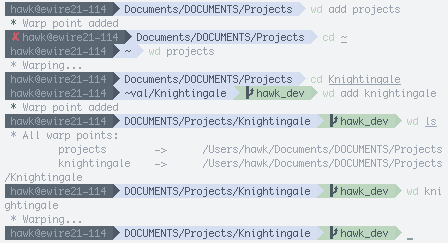
\includegraphics[resolution=72, scale=0.75]{Lab1Images/demos/wd.png}
			\caption{Demonstrating the use of the `wd' plugin}
			\label{wd}
		\end{figure}

		\begin{figure}[!htb]
			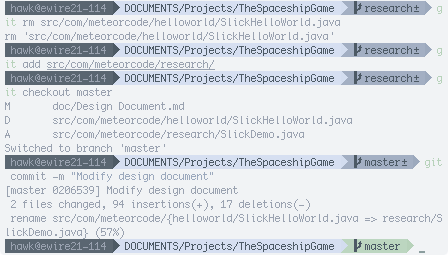
\includegraphics[resolution=72, scale=0.75]{Lab1Images/demos/gitdemo.png}
			\caption{Demonstrating the use of a customized prompt to display Git repository information}
			\label{git}
		\end{figure}
		\FloatBarrier
	\section{A description of the challenges that you encountered while customizing and using zsh}

		I did not encounter any major difficulties customizing and using zsh. The documentation for the fish-like plugins ``zsh-history-substring-search'' and ``zsh-autosuggestions'' did not assume that users have oh-my-zsh installed, but adapting their installation instructions for an environment with oh-my-zsh installed was not a significant challenge.

		I did encounter some problems related to formatting my laboratory report in \LaTeX, mostly related to using Unix commands, .zshrc property names, and paths, all of which included characters that \LaTeX\ requires to be escaped. I eventually solved these problems by using a \lstinline!\lstinline! environment from the \lstinline{listings} package, which I modified slightly to display listings in teletype font, as is the convention for source code and Unix commands, and to ensure that listings wrap lines without hyphenation, as adding hyphens would add incorrect information to the Unix commands.

\end{document}